\documentclass[12pt,letterpaper,boxed]{hmcpset}
\usepackage[margin=1in,headheight=14pt]{geometry}
\usepackage{amsfonts, amsmath, amssymb, enumerate, fancyhdr, gensymb, lastpage, mathtools, parskip, graphicx}
\usepackage{xcolor, tikz-cd}
\newcommand{\wg}[1]{\textcolor{violet}{#1}}
\newcommand{\OO}{\mathcal O}
\newcommand{\Q}{\mathbb Q}
\newcommand{\R}{\mathbb R}
\newcommand{\C}{\mathcal C}
\newcommand{\Z}{\mathbb Z}
\newcommand{\abs}[1]{\left|#1\right|}
\newcommand{\im}{\text{im }}
\newcommand{\inv}{^{-1}}
\usepackage[shortlabels]{enumitem}

% Numbering macros
\pagestyle{fancy}
\lhead{Will Gilroy}
\chead{Algs Homework \#}
\rhead{03 November 2021}
\lfoot{}
\cfoot{}
\rfoot{Page\ \thepage\ of\ \pageref{LastPage}}

\linespread{1.5}

\newcommand\blankpage{
    \thispagestyle{empty}
    \addtocounter{page}{-1}
    \newpage}
\renewcommand\footrulewidth{0.4pt}

\begin{document}

\problemlist{Algorithms HW } 

%------------------------- Problem 1 -----------------------

\begin{problem}
	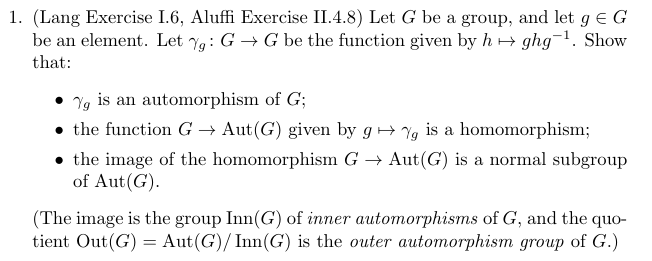
\includegraphics[scale=0.9]{1.png}
	\hfill
\end{problem}

\begin{solution}
\begin{enumerate}
	\item We show that $\gamma_g$ is a bijective homomorphism, for
	some fixed $g \in G$.
	Let $k, \ell \in G$ then we have \[
	\gamma_g(k \cdot \ell) = g \cdot
	(k \cdot \ell) \cdot g\inv = g \cdot k \cdot e \cdot \ell \cdot
	g\inv = (g \cdot k \cdot g\inv) \cdot (g \cdot \ell \cdot g\inv) =
	\gamma_g(k) \cdot \gamma_g(\ell),
	\]
	since group products are associative and by definition of the
	identity element. Hence $\gamma_g$ is a homomorphism for all $g
	\in G$.

	Now suppose $\gamma_g(h) = e$ for some $h \in G$ we have 
	\begin{align*}
		\gamma_g(h) &= e \\
		ghg\inv &= e \\
		(g\inv g)h(g\inv g) &= g\inv e g\\
		h &= g\inv e g \\ 
		h &= e.
	\end{align*} 
	Thus, $\gamma_g(h)$ is injective. Now let $k \in G$ and notice
	that $\gamma_g(g\inv k g) = g\cdot g\inv k g\inv g = k$. Moreover,
	$g\inv k g \in G$ since $G$ is closed under its group operation.
	That is, $\gamma_g$ is surjective for all $g \in G$.
	Hence, we have shown that $\gamma_g$ is an automorphism of $G$.

	\item Let $g,h \in G$.
	And let $f: G \to Aut(G)$ be the map $f(g)
	= \gamma_g$. 
	
	Consider the action of $\gamma_{gh}$ on
	some group element $k$. We have
	\begin{align*}
		\gamma_{gh}(k) &= (gh) k (gh)\inv \\
			&= (gh) k (h\inv g\inv) \\ 
			&= g (h k h\inv) g\inv \\
			&= (\gamma_g \circ \gamma_h)(k),
	\end{align*}
	holds for all $k \in G$. That is, we have shown $f(g \cdot h) = f(g)
	\circ f(h)$, where $\cdot$ denotes the product in $G$ and $\circ$
	denotes function composition --- the group operation in $Aut(G)$.
	Hence, $f$ is a homomorphism

	\item We show directly that $\im f$ is closed under conjugation by
	homomorphism in $Aut(G)$. Let $h \in Aut(G)$ and $\gamma_g \in \im
	f$. There then exists an
	inverse homomorphism $h\inv$ and consider the action of \[
		h \circ \gamma_g \circ h\inv.
	\]
	This is an automorphism since the composition of group
	homomorphisms is again a group homomorphism \wg{check this}.

	Let $k \in G$ and consider 
	\begin{align*}
		(h \circ \gamma_g \circ h\inv)(k) &= h(g \cdot h\inv(k) \cdot g\inv) \\
			&= h(g) \cdot k \cdot h(g\inv), && \text{since $h$ is a homomorphism}
	\end{align*}
	Moreover, $h(g) = g' \in G$ since $h$ is an automorphism of $G$.
	That is, we have shown $(h \circ \gamma_g \circ g\inv) = f(g') \in
	\im f$. And so, $\im f$ is a normal sunbgroup of $Aut(G)$ by
	definition.

\end{enumerate}
\end{solution}

\newpage

%------------------------- Problem 2 -----------------------

\begin{problem}[2]
	\hfill
\end{problem}

\begin{solution}
\end{solution}

\newpage

%------------------------- Problem 3 -----------------------

\begin{problem}[3]
	\hfill
\end{problem}
\begin{solution}
\end{solution}

\newpage

%------------------------- Problem 4 -----------------------

\begin{problem}[4]
	\hfill
\end{problem}

\begin{solution}
\end{solution}

\newpage


%------------------------- Problem 5 -----------------------

\begin{problem}[1]
	\hfill
\end{problem}

\begin{solution}
\end{solution}

\newpage

%------------------------- Problem 6 -----------------------

\begin{problem}[1]
	\hfill
\end{problem}

\begin{solution}
\end{solution}

\newpage

%------------------------- Problem 7 -----------------------

\begin{problem}[1]
	\hfill
\end{problem}

\begin{solution}
\end{solution}

\newpage

\end{document}
